\section{CERN and the LHC}
\subsection{The European Organisation for Nuclear Research CERN}
CERN is the European Organisation for Nuclear Research. The name is derived from the french
acronym for Conseil Europeen pour la Recherche Nucleaire, or European Council for Nuclear
Research.

\subsection{The LHC Machine}
The Large Hadron Collider \cite{LHC} at CERN is the most power tool for particle physics studies. 
The CERN accelerator complex, shown in Figure~\ref{CERNcomplex}, comprises the Linear
Accelerator, LINAC, the Proton Synchrotron, PS, and the Super Proton Synchrotron,
	SPS, which form a chain of successively energetic accelerators. The energies reached by the protons at the end of each accelerator are:
\begin{itemize}
	\item	Proton LINear ACcelerator (LINAC): Up to 50 MeV
	\item Proton Synchrotron Booster (PSB) : 1.4 GeV
	\item Proton Synchrotron (PS) : 26 GeV
 	\item Super Proton Synchrotron (SPS): 450 GeV
	\item LHC: 7 TeV
\end{itemize}
The accelerator tunnel comprises eight straight sections and eight arcs, as shown in .
The tunnel contains the two rings which produce two counter-rotating particle beams colliding 
at Points 1, 2, 5 and 8, where the ATLAS, ALICE, CMS and LHCb experiments are located, respectively. 
The beam is accelerated using the Radio-Frequency (RF) cavities located in the straight section at Point 4, while Points 3 and 7 contain beam
collimation systems which shape and clean the beam. The straight section in Point 6 is used as the beam dump, where the beams are removed from 
the LHC and ”dumped” into a graphite target to dissipate the beam’s energy.

%four interaction points. The four main detectors are built around these points.

The arcs are built using a total of 1232 superconducting dipole magnets which keep the beams
in the (nearly) circular orbit. Each of the dipole magnets is capable of generating a magnetic field
of up to 8 T. Additionally, there are 392 quadrapole magnets, located in the straight sections, which
serve to focus the beam.

\begin{figure}[htbp]
%\vspace{0.5cm}
%\setcapindent{2em}
  \centering
	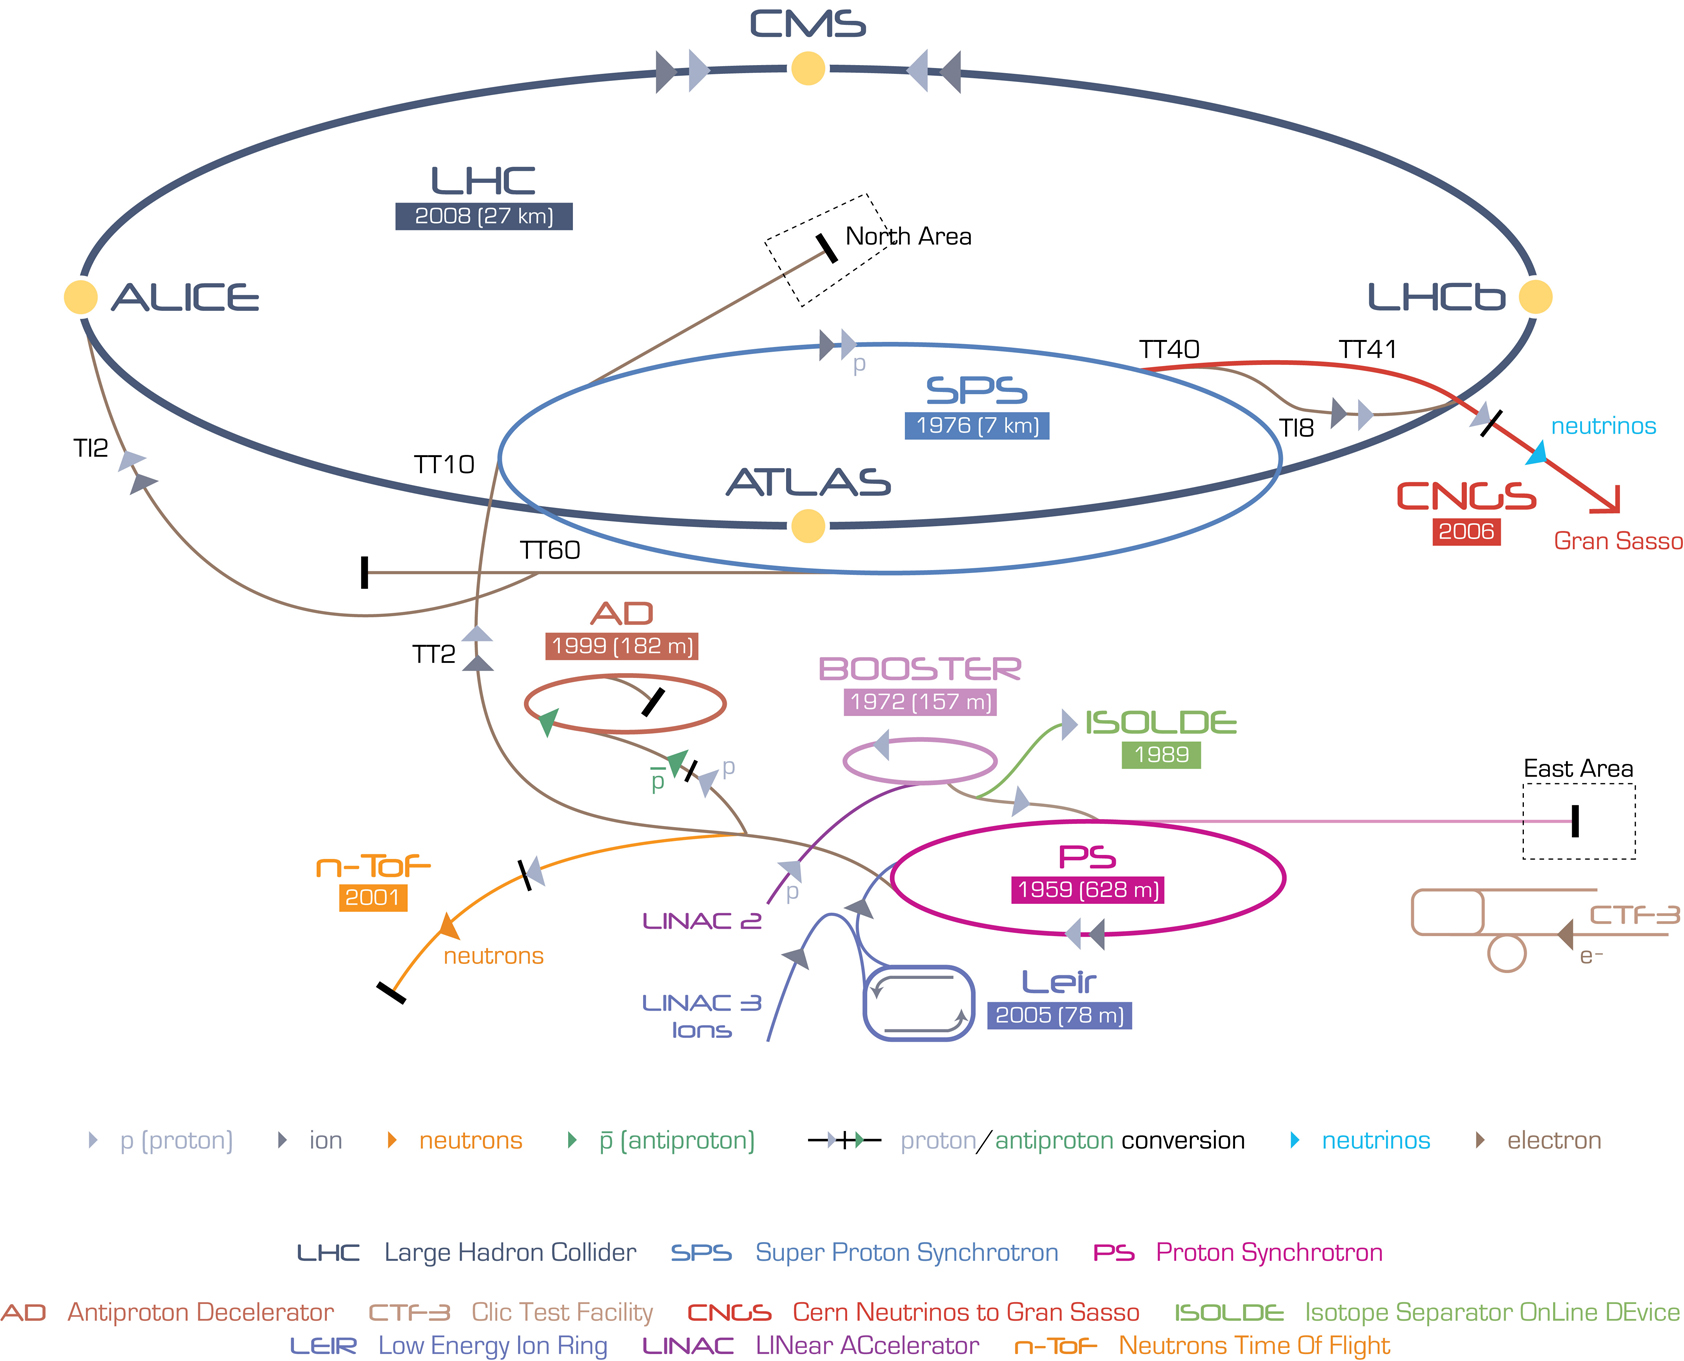
\includegraphics[width=0.9\textwidth]{cern_atlas/Cern-Accelerator-Complex.jpg}
	\caption[CERN accelerator complex]{CERN accelerator complex}
	\label{CERNcomplex}
\end{figure}
\subsubsection{Accelerator and Energy}
Figure~\ref{lhc-dipole}
\begin{figure}[htbp]
  \centering
  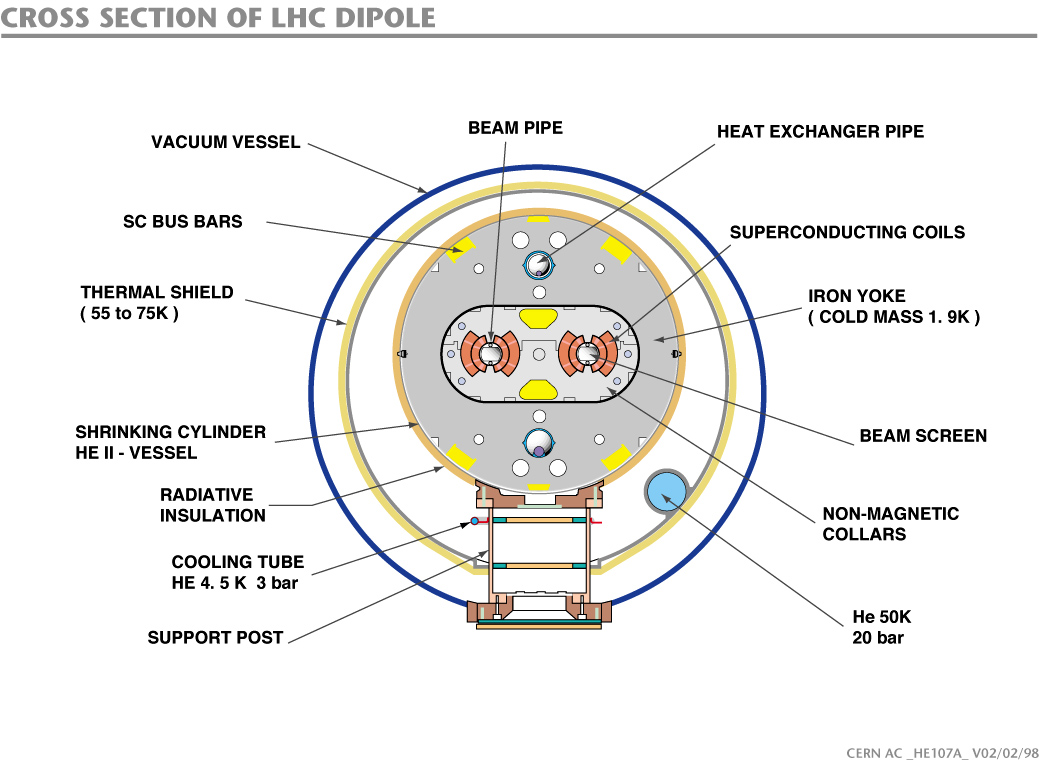
\includegraphics[width=0.9\textwidth]{cern_atlas/lhc-dipole.jpg}
  \caption[lhc-dipole]{lhc-dipole}
  \label{lhc-dipole}
\end{figure}
\subsubsection{The Experiments on the LHC}
The experiments installed on the LHC ring are briefly decribed below:
Figure~\ref{lhc-exp}
\\
{\bf ALICE} {\it (A Large Ion Collider Experiment)} \cite{ALICE}:
\\
{\bf ATLAS} {\it (A Toroidal LHC Apparatus)} \cite{ATLAS}:
\\
{\bf CMS} {\it (Compact Muon Solenoid)} \cite{CMS}:
\\
{\bf LHCb} {\it (Large Hadron Collider beauty)} \cite{LHCb}:
\\

{\bf LHCf} \cite{LHCf} :
The Large Hadron Collider forward experiment is the smallest of all the LHC experiments. Its aim is to study the particles generated in the forward region of collisions,	to verify hadronic models at very high energy for the understanding of ultra-high energetic cosmic rays. It consists of two small detectors, 140 m on either side of the ATLAS intersection point.
\\

{\bf TOTEM} \cite{TOTEM}:
The TOTEM experiment measures the total pp cross section and study
elastic scattering and diffractive dissociation at the LHC. TOTEM also aims to measure
the luminosity at the CMS interaction point where it is based. It covers the
very forward region in the pseudo-rapidity range.
\\

\begin{figure}[htbp]
  \centering
  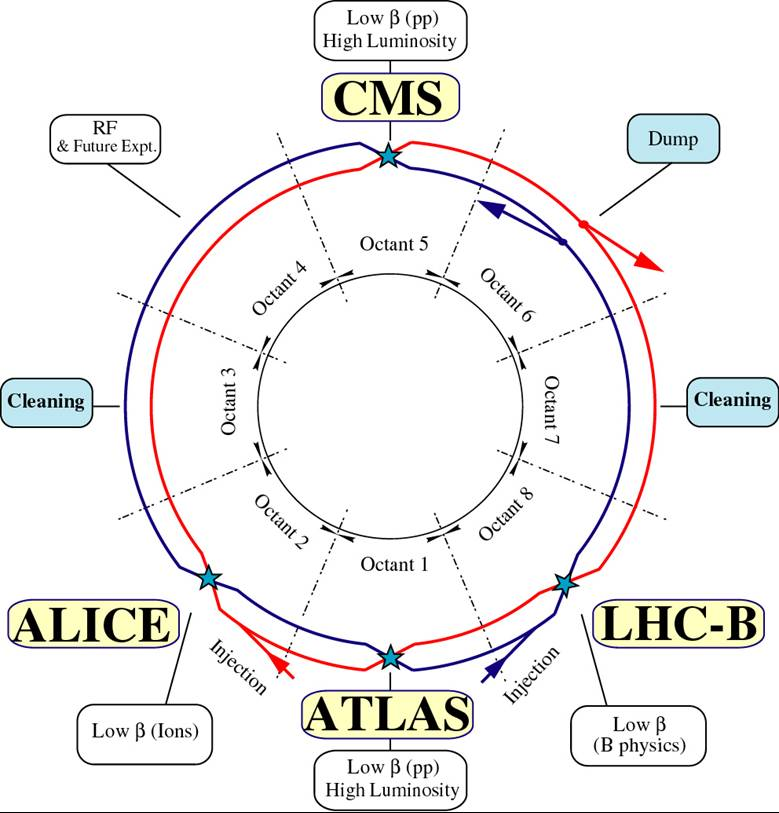
\includegraphics[width=0.7\textwidth]{cern_atlas/lhc-schematic.jpg}
  \caption[lhc-exp]{lhc-exp}
  \label{lhc-exp}
\end{figure}

\newpage
\section{The ATLAS Detector}
Figure~\ref{ATLAS}
\begin{figure}[htbp]
  \centering
  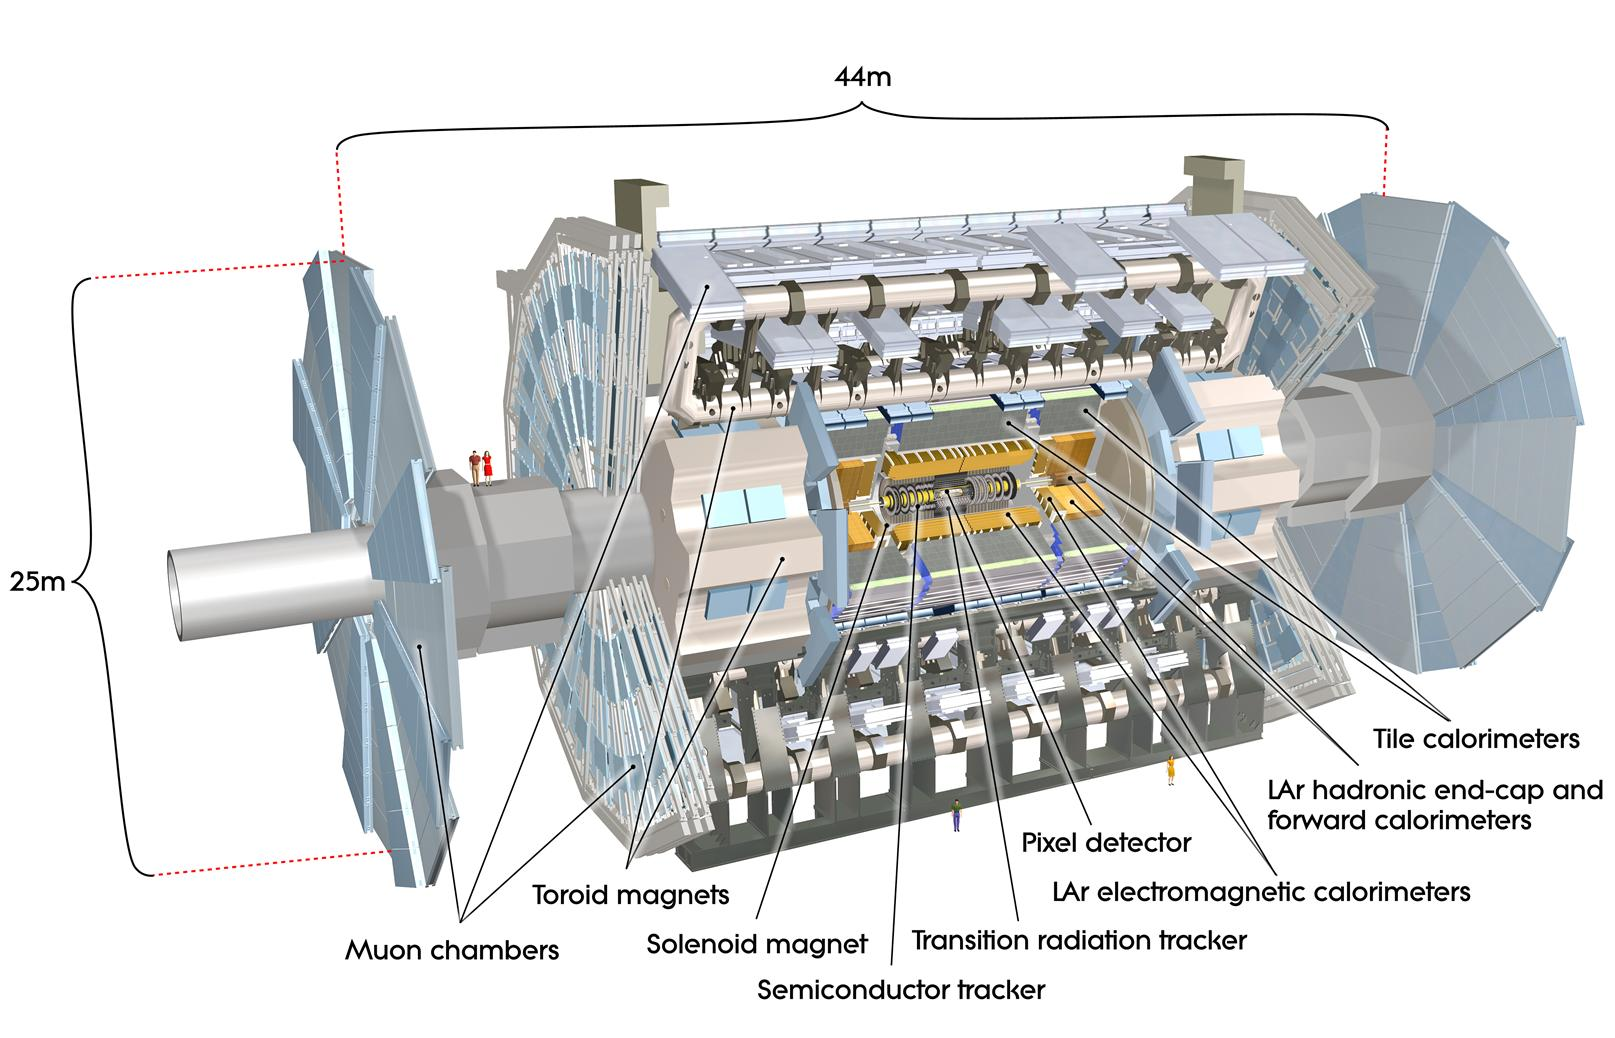
\includegraphics[width=0.9\textwidth]{cern_atlas/ATLAS.jpg}
  \caption[ATLAS]{ATLAS}
  \label{ATLAS}
\end{figure}


\subsection{The Inner detector}
Figure~\ref{InnerDetector}
\begin{figure}[htbp]
  \centering
  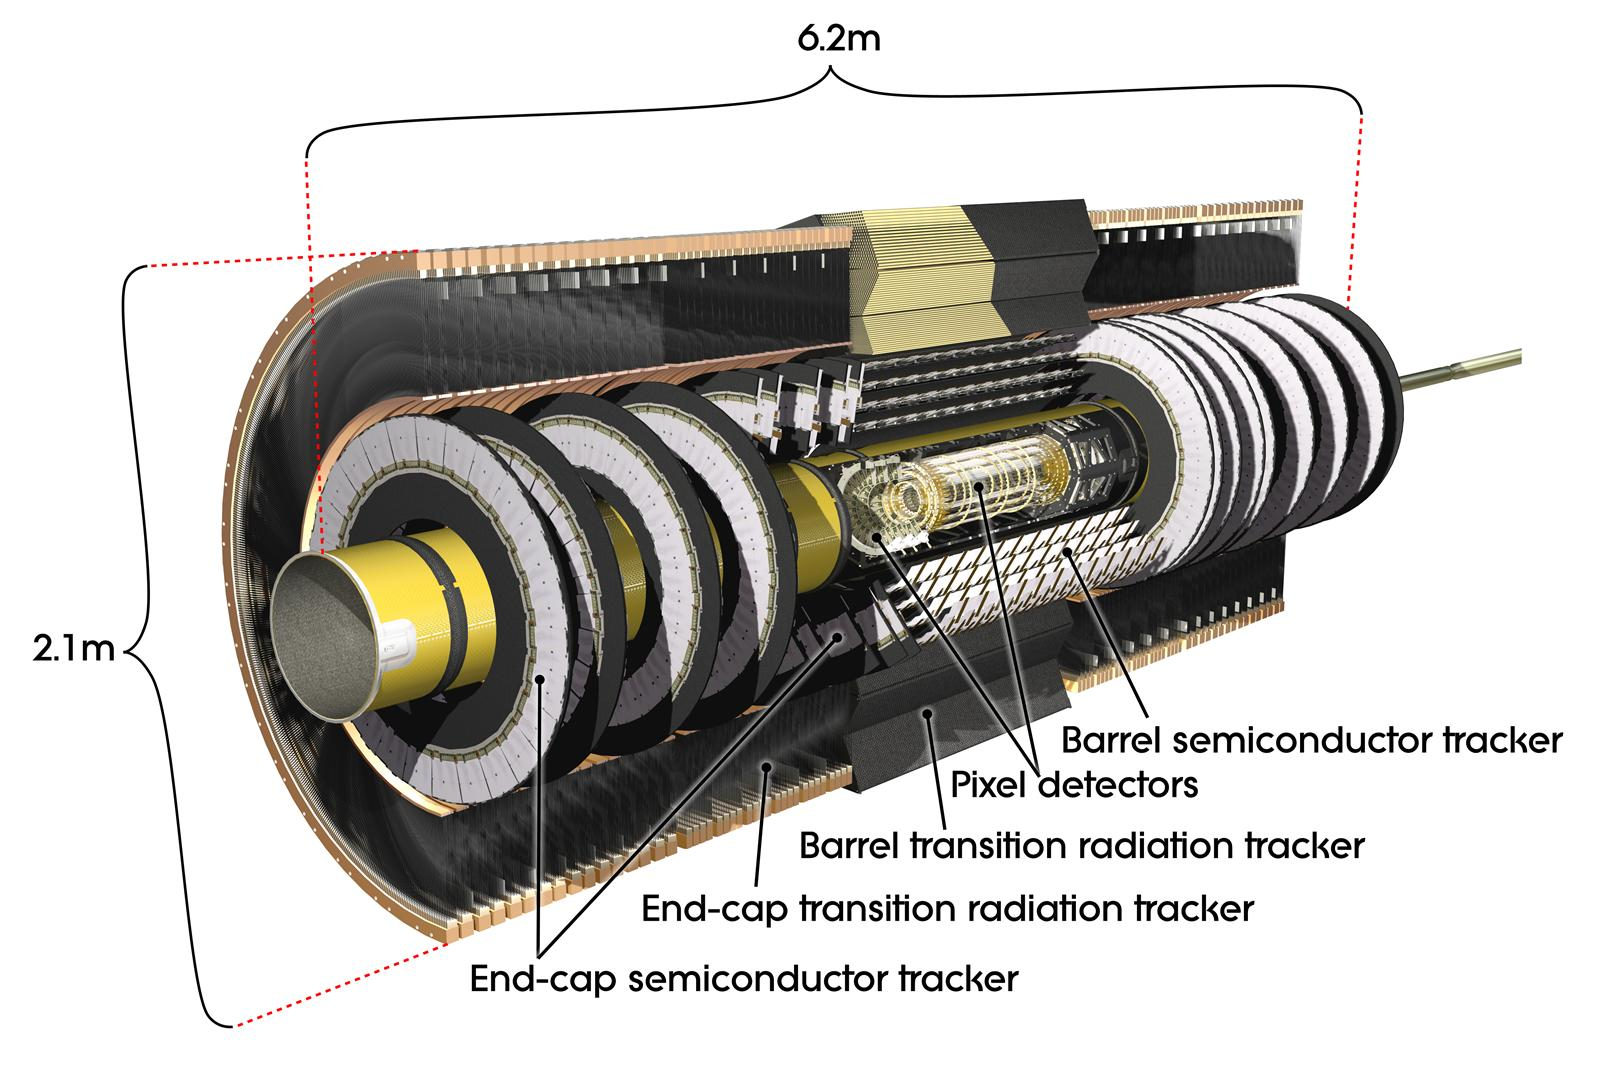
\includegraphics[width=0.8\textwidth]{cern_atlas/InnerDetector.jpg}

  \caption[ATLAS]{ATLAS}
  \label{InnerDetector}
\end{figure}


Figure~\ref{pixel}
\begin{figure}[htbp]
  \centering
  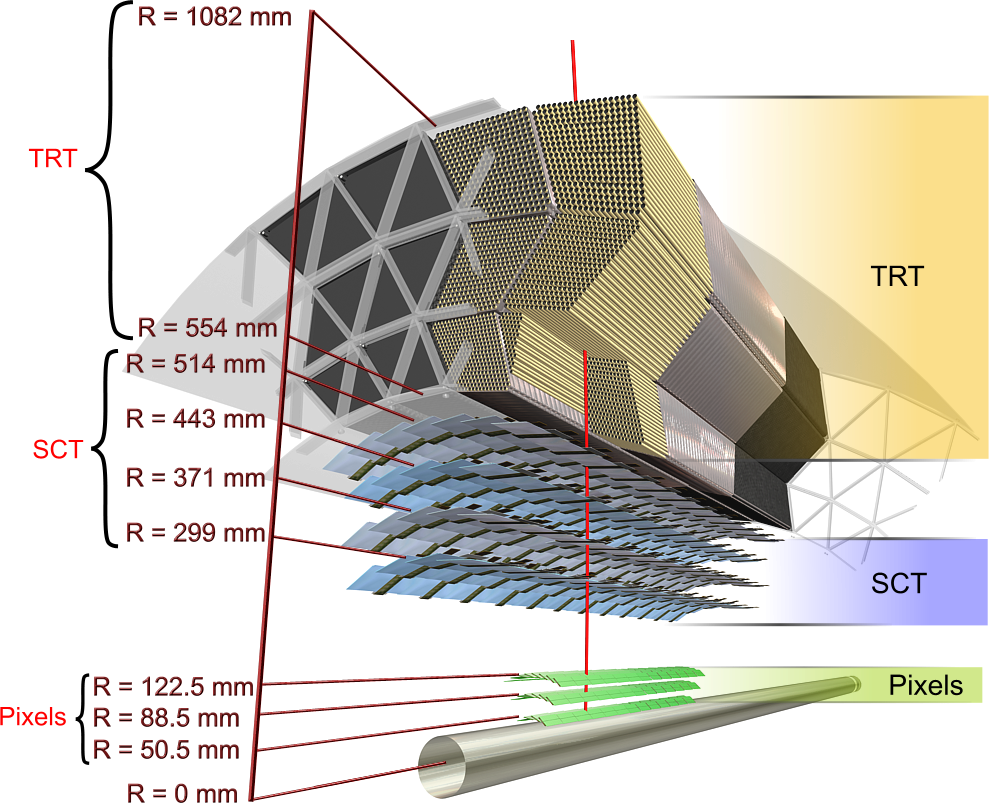
\includegraphics[width=0.65\textwidth]{cern_atlas/pixel_01.png}
	%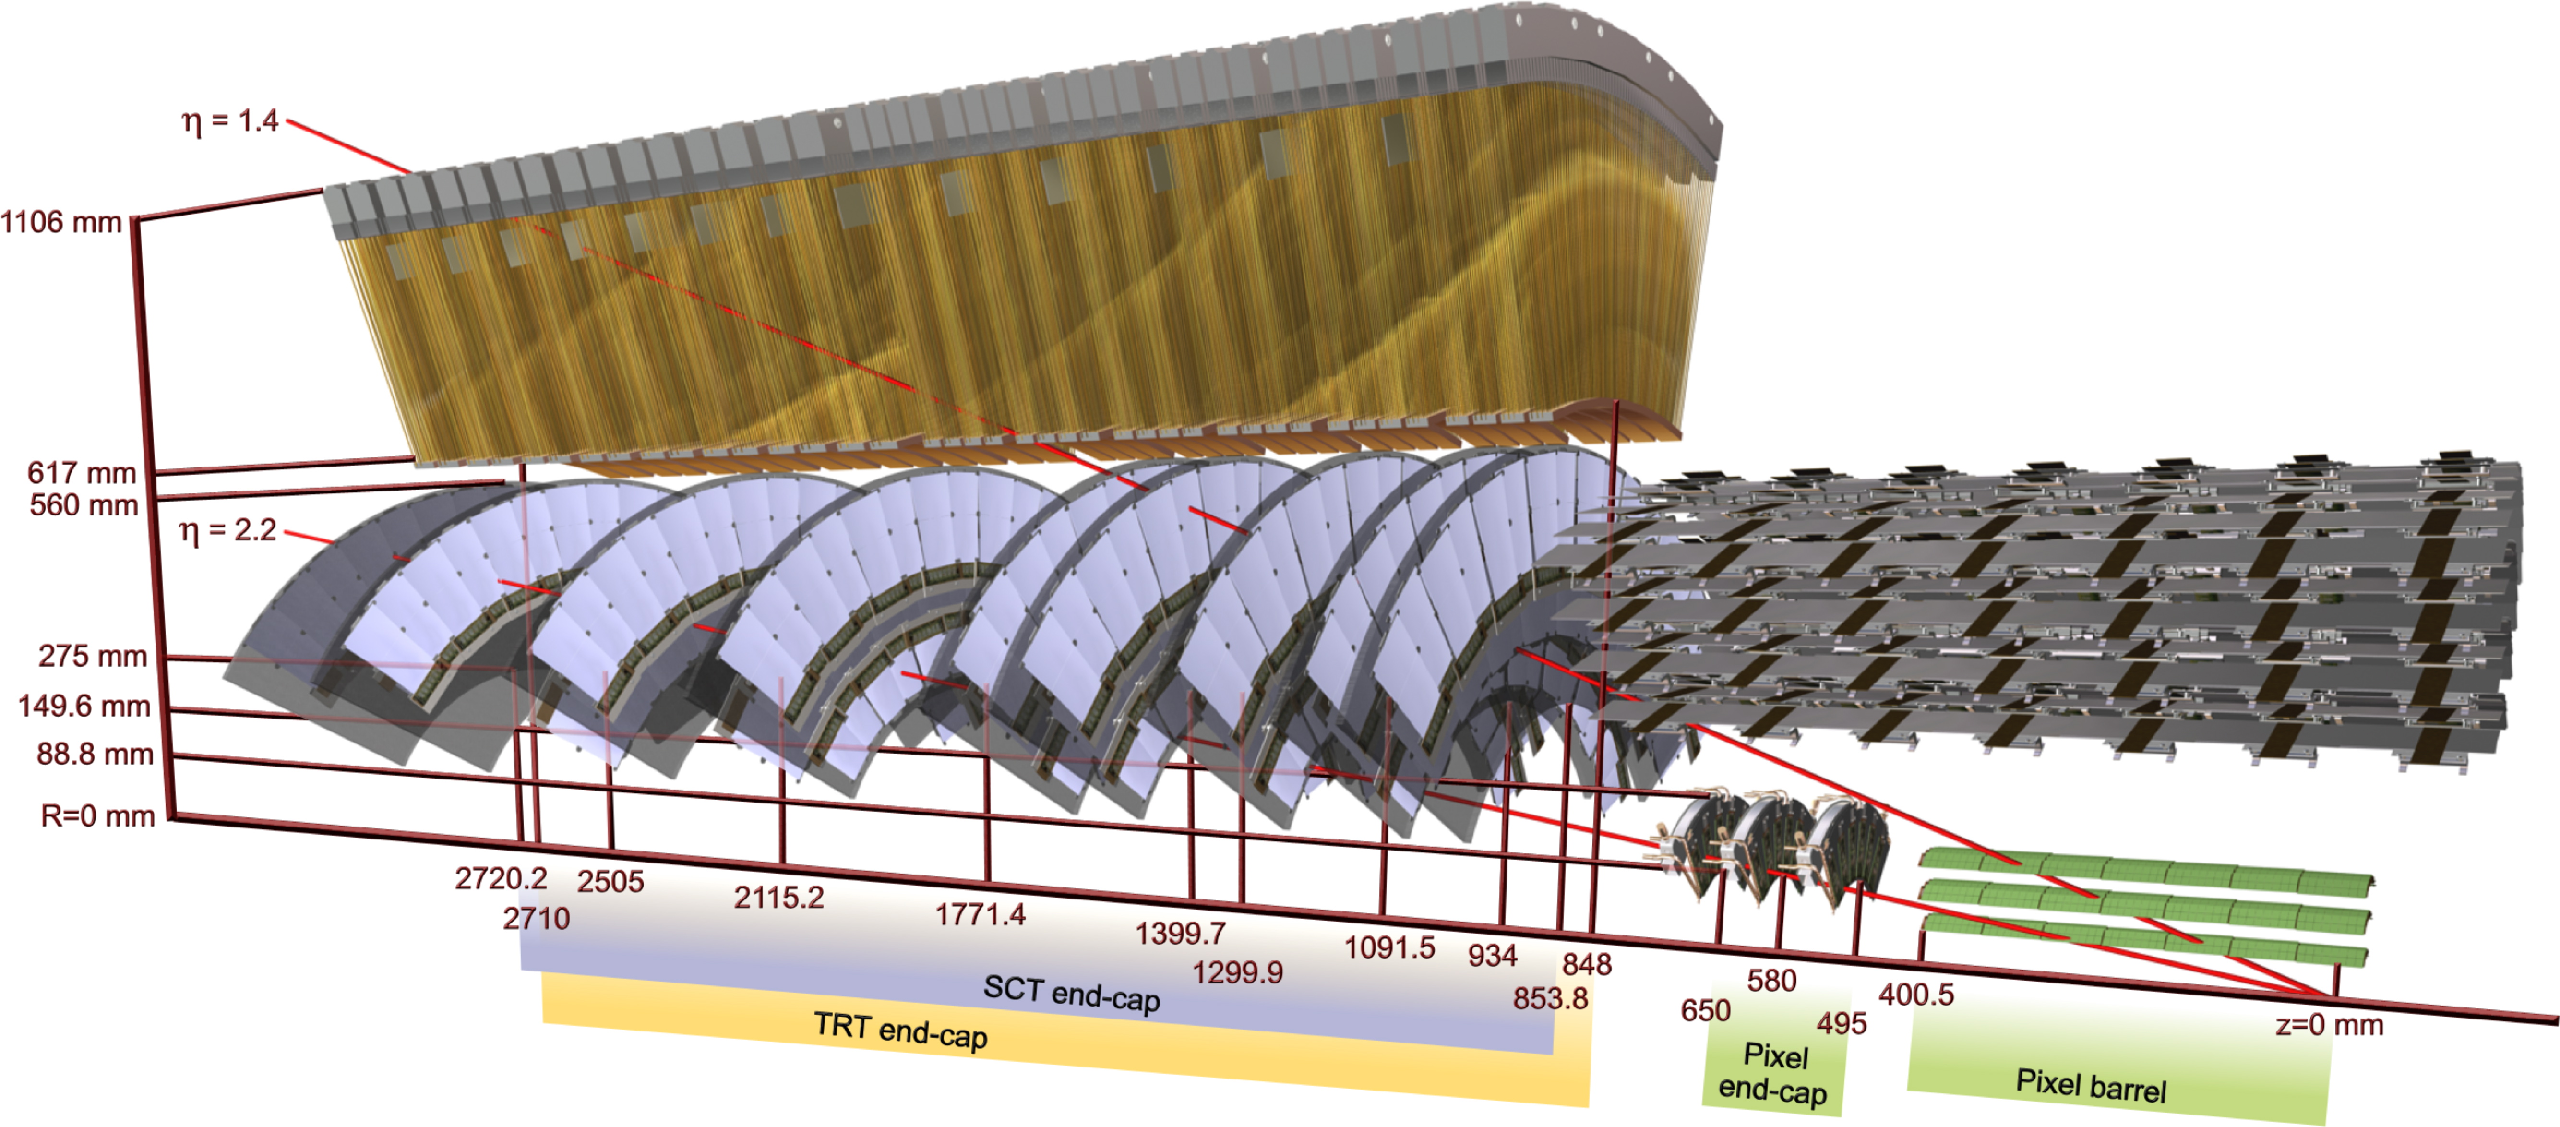
\includegraphics[width=0.48\textwidth]{cern_atlas/pixel_02.png}
  \caption[ATLAS]{ATLAS}
  \label{pixel}
\end{figure}


\subsubsection{The Insertable B-Layer (IBL)}
\subsubsection{The silicon Pixel detector}
\subsubsection{The SemiConductor Tracker (SCT)}
\subsubsection{The Transition Radiation Tracker (TRT)}

\subsection{The calorimeters}
Figure~\ref{calo}
\begin{figure}[htbp]
  \centering
  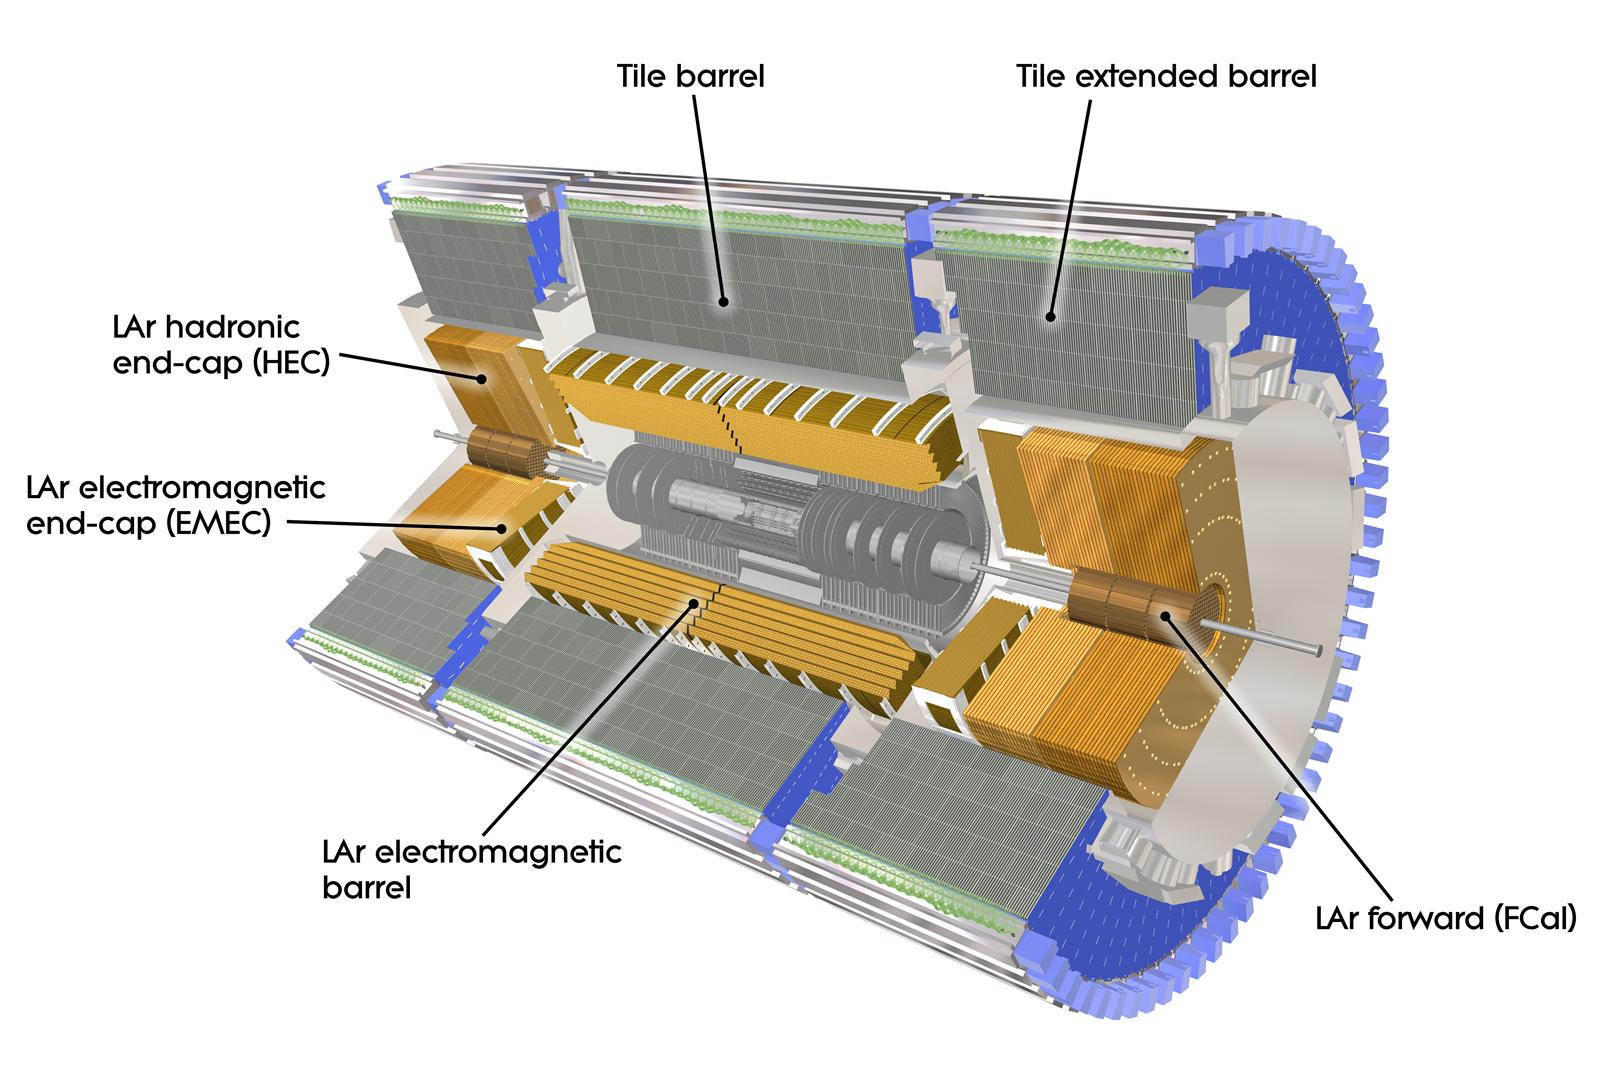
\includegraphics[width=0.8\textwidth]{cern_atlas/calorimeter.jpg}
	%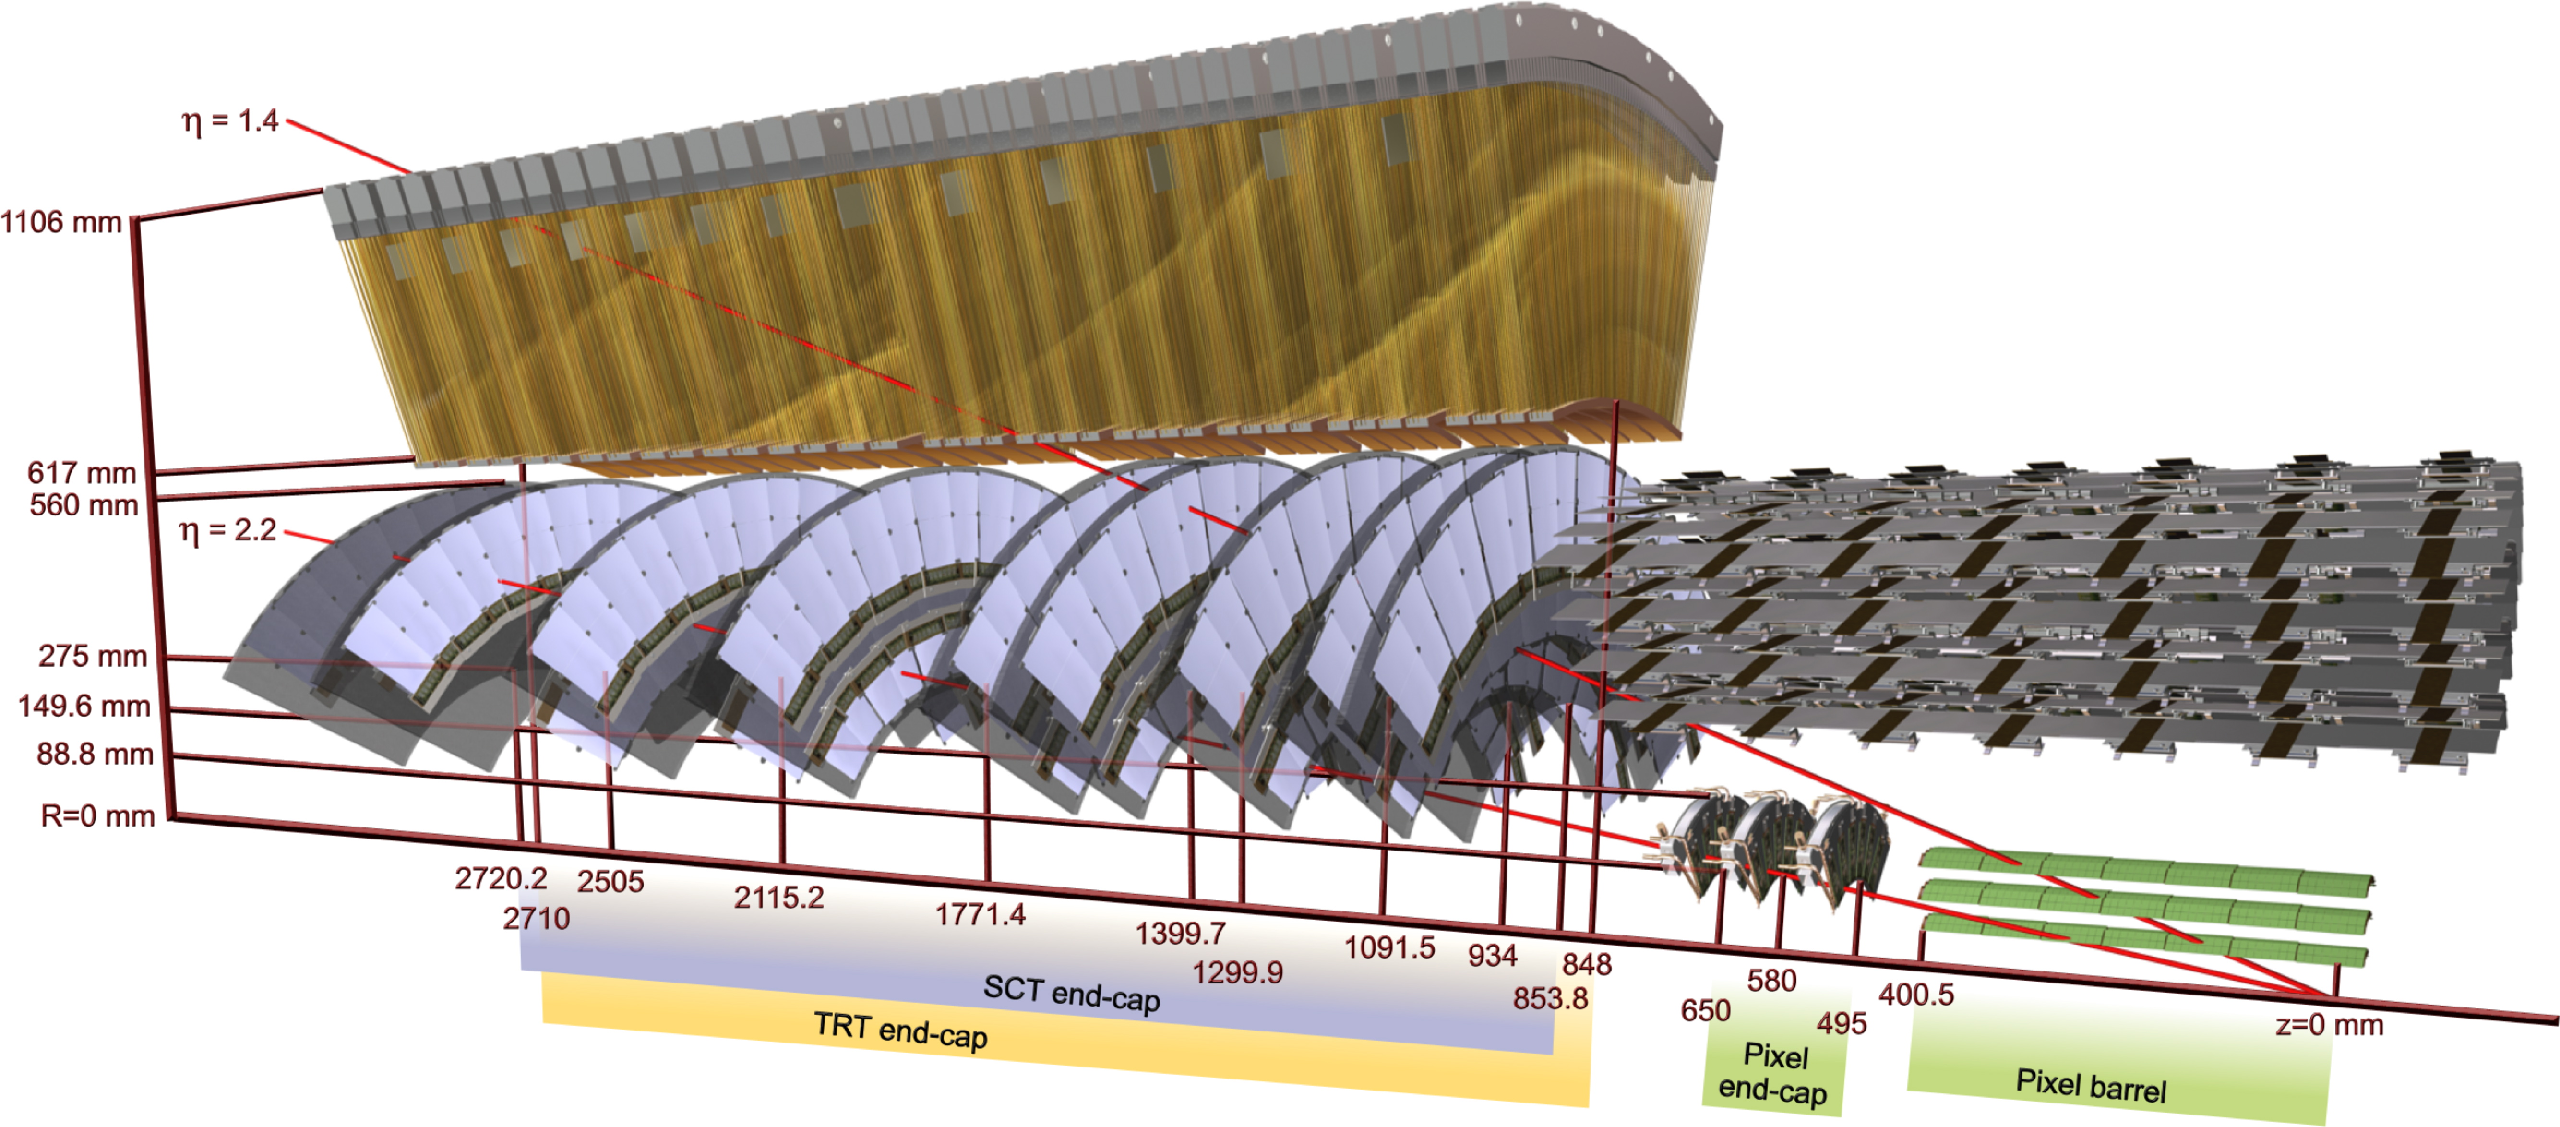
\includegraphics[width=0.48\textwidth]{cern_atlas/pixel_02.png}
  \caption[ATLAS]{ATLAS}
  \label{calo}
\end{figure}


\subsubsection{The electromagnetic calorimeter}
Figure~\ref{caloLAr}
\begin{figure}[htbp]
  \centering
  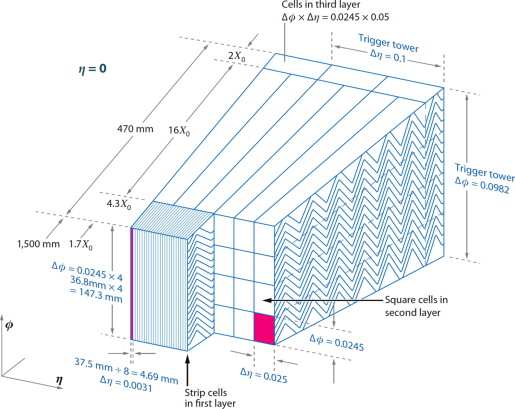
\includegraphics[width=0.48\textwidth]{cern_atlas/cellLAr.jpg}
	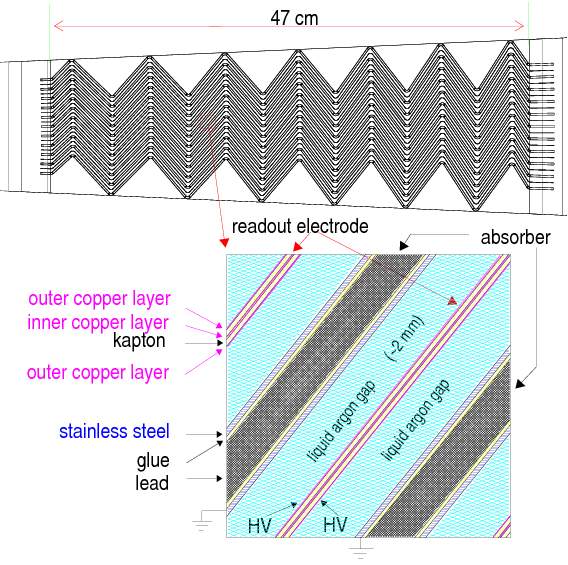
\includegraphics[width=0.48\textwidth]{cern_atlas/larg_principle.png}
  \caption[ATLAS]{ATLAS}
  \label{caloLAr}
\end{figure}

\subsubsection{Hadronic calorimeter}


\subsection{The muon spectrometer}
Figure~\ref{MuonSys}
\begin{figure}[htbp]
  \centering
  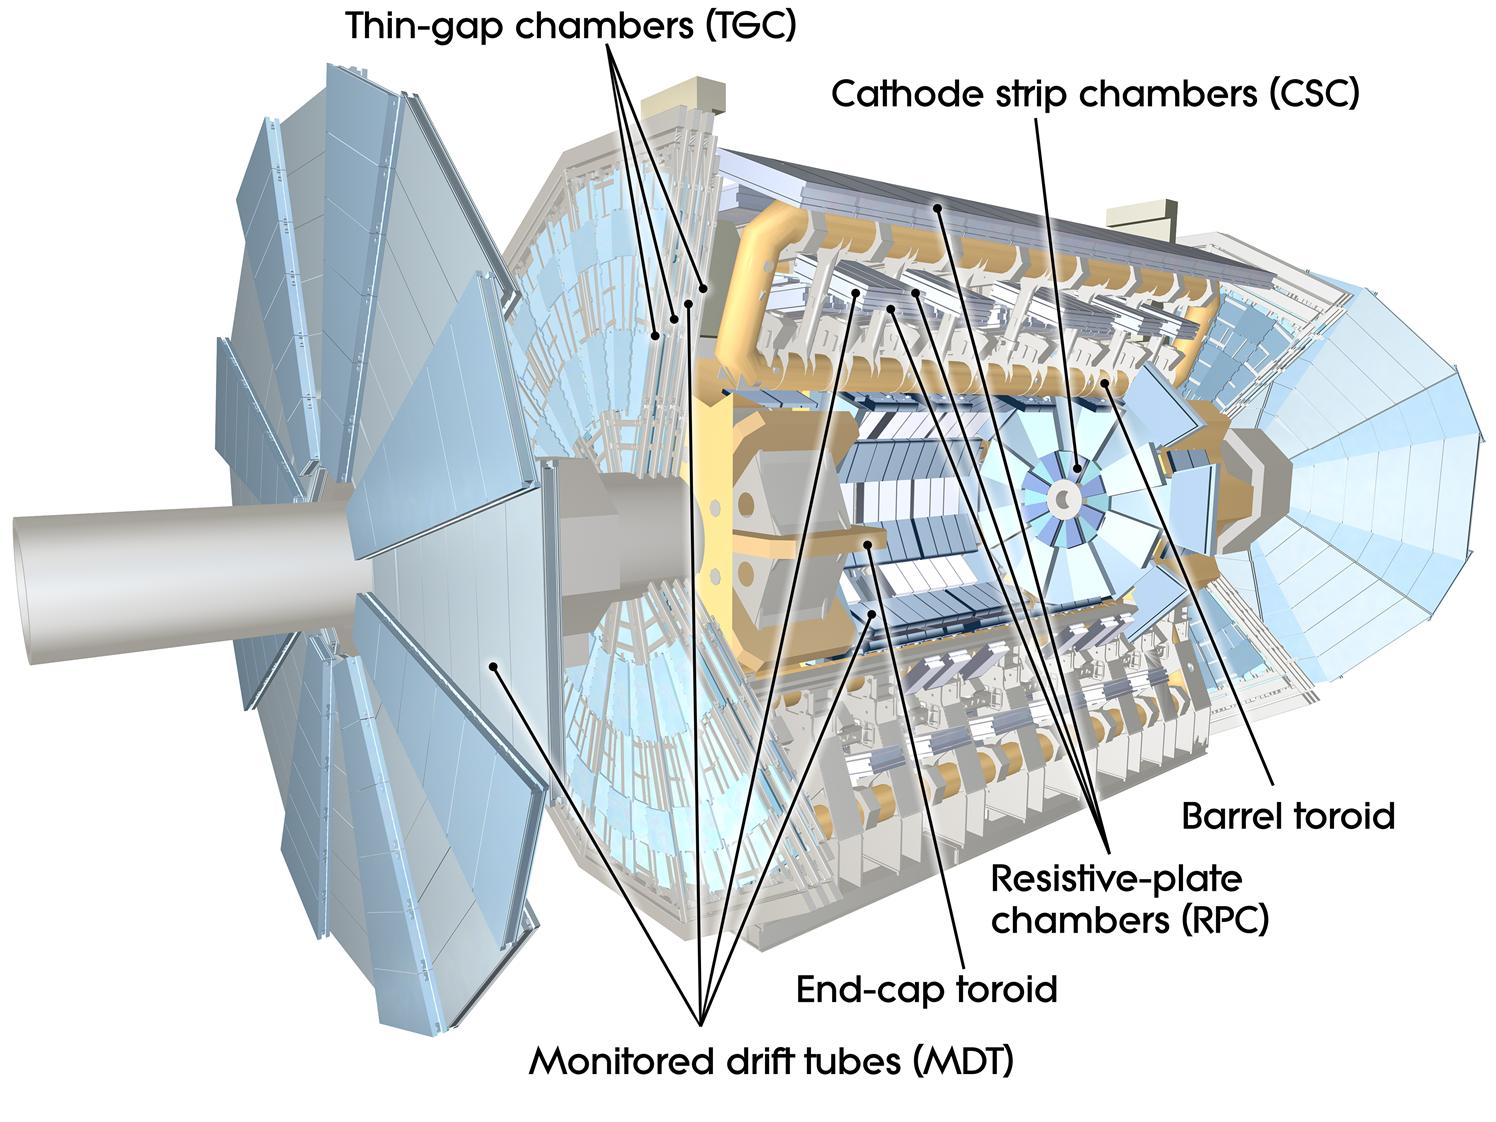
\includegraphics[width=0.7\textwidth]{cern_atlas/MuonSystem.jpg}
  \caption[ATLAS]{ATLAS}
  \label{MuonSys}
\end{figure}

\section{The ATLAS trigger system}
\section{}

